\documentclass[12pt,a4paper]{article}
\usepackage[utf8]{inputenc}
\usepackage[spanish,es-tabla]{babel}
\usepackage{geometry}
\usepackage{graphicx}
\usepackage{multirow}
\usepackage{tabularx}
\usepackage{mathptmx}
\usepackage{fancyhdr}
\usepackage{array}
\usepackage[table]{xcolor}
\usepackage{titlesec}
\usepackage{setspace}
\usepackage{microtype}
\usepackage{lastpage}
\usepackage{booktabs}
\usepackage{enumitem}
\usepackage{amsmath}
\usepackage{amsfonts}
\usepackage{amssymb}

\graphicspath{{images/}{../images/}{./}}

\geometry{
    top=4.7cm,
    bottom=2.5cm,
    left=2.5cm,
    right=2.5cm,
    headheight=3.9cm,
    headsep=0.4cm
}

\setstretch{1.15}
\setlength{\parindent}{0pt}
\setlength{\parskip}{0.45em}
\setlength{\tabcolsep}{4pt}

\titleformat{\section}
  {\normalfont\fontsize{12}{14.5}\bfseries}{\thesection.}{0.6em}{\uppercase}
\titlespacing*{\section}
  {0pt}{1.8ex plus 0.4ex minus 0.2ex}{0.6ex plus 0.2ex}

\titleformat{\subsection}
  {\normalfont\fontsize{11.5}{13.5}\bfseries}{\thesubsection.}{0.5em}{}
\titlespacing*{\subsection}
  {0pt}{1.4ex plus 0.3ex minus 0.1ex}{0.4ex plus 0.1ex}

\titleformat{\subsubsection}
  {\normalfont\fontsize{10.5}{12.5}\bfseries\itshape}{\thesubsubsection.}{0.4em}{}
\titlespacing*{\subsubsection}
  {0pt}{1.1ex plus 0.2ex minus 0.1ex}{0.3ex plus 0.1ex}

\newcolumntype{Y}{>{\centering\arraybackslash}X}
\newcolumntype{L}{>{\raggedright\arraybackslash}X}
\newcolumntype{C}{>{\centering\arraybackslash}X}

\definecolor{headerblue}{RGB}{26, 54, 93}
\definecolor{darkblue}{RGB}{43, 108, 176}
\definecolor{lightgraybg}{RGB}{248, 248, 248}
\definecolor{tableheader}{RGB}{232, 238, 246}

\newcommand{\docCodigo}{TI-SIGE-ENT-F1-003}
\newcommand{\docVersion}{1.0}
\newcommand{\docProceso}{INGENIERÍA DE REQUERIMIENTOS / ESPECIFICACIÓN FORMAL}
\newcommand{\docElaboracion}{21/08/2026}
\newcommand{\docRevision}{21/08/2026}
\newcommand{\docTitulo}{DEFINICIÓN DE REQUISITOS FUNCIONALES Y NO FUNCIONALES}
\newcommand{\docOrganizacion}{FACULTAD DE INGENIERÍA EN SISTEMAS, ELECTRÓNICA E INDUSTRIAL}
\newcommand{\docSubOrganizacion}{CARRERA DE INGENIERÍA DE SOFTWARE}

\newcommand{\encabezadofrecuente}{%
    \renewcommand{\arraystretch}{1.15}%
    \noindent\makebox[\textwidth][c]{%
    \begin{tabularx}{\textwidth}{|>{\centering\arraybackslash}m{2.8cm}|Y|>{\centering\arraybackslash}m{4.8cm}|}
        \hline
        \multirow{4}{2.8cm}{\centering\raisebox{-1.15cm}{
\includegraphics[width=2.5cm,height=2.0cm,keepaspectratio]{images/logo.png}}}
        & \textbf{\fontsize{9}{11}\selectfont \docOrganizacion} 
        & \textbf{\fontsize{8}{10}\selectfont CÓDIGO:} \fontsize{8}{10}\selectfont \docCodigo \\
        \cline{3-3}
        & \textbf{\fontsize{8.5}{10.5}\selectfont \docSubOrganizacion} 
        & \textbf{\fontsize{8}{10}\selectfont VERSIÓN:} \fontsize{8}{10}\selectfont \docVersion \\
        \cline{2-3}
        & \textbf{\fontsize{8}{10}\selectfont PROCESO:} \fontsize{8}{10}\selectfont \docProceso 
        & \textbf{\fontsize{8}{10}\selectfont ELABORACIÓN:} \fontsize{8}{10}\selectfont \docElaboracion \\
        \cline{2-3}
        & \textbf{\fontsize{8.5}{10.5}\selectfont \docTitulo} 
        & \textbf{\fontsize{8}{10}\selectfont ÚLTIMA REVISIÓN:} \fontsize{8}{10}\selectfont \docRevision \\
        \hline
    \end{tabularx}%
    }%
}

\pagestyle{fancy}
\fancyhf{}
\fancyhead[C]{\encabezadofrecuente}
\fancyfoot[C]{\fontsize{10}{12}\selectfont Página \thepage\ de \pageref{LastPage}}
\renewcommand{\headrulewidth}{0pt}

\begin{document}

\noindent{\fontsize{10.5}{12.5}\selectfont \textbf{Integrantes:} Heidi Villavicencio \quad$\vert$\quad Steeven Toala \quad$\vert$\quad Nixon Hurtado \quad$\vert$\quad Andrea Vásquez}

\vspace{0.25cm}

\section{Título}
\textbf{Denominación del Entregable:} Especificación de Requisitos de Software (SRS IEEE 830) -- Código EDT: 1.3

\section{Introducción}
La especificación rigurosa de los requerimientos constituye el cimiento para el diseño y construcción del sistema SIGE. Siguiendo el estándar internacional IEEE 830 y los lineamientos de calidad ISO/IEC 25010, se formalizan en este informe los 24 requerimientos funcionales (RF-01 a RF-24) y 10 requerimientos no funcionales (RNF-01 a RNF-10) que rigen la arquitectura y el comportamiento del software. Cada requerimiento ha sido clasificado por módulo de negocio y ponderado por criticidad para garantizar la completa digitalización de los formatos SGC \texttt{P7-T1} y \texttt{P7-T2}.

\section{Objetivo}
\subsection{Objetivo General}
Especificar de manera formal, completa y verificable los requisitos funcionales y no funcionales del sistema SIGE bajo el estándar IEEE 830, alineados con el Sistema de Gestión de Calidad institucional de la FISEI.
\subsection{Objetivos Específicos}
\begin{itemize}[leftmargin=1.5em, itemsep=2pt]
    \item Formalizar los 24 requerimientos funcionales estructurados en 7 módulos del sistema.
    \item Definir los 10 requisitos no funcionales bajo las dimensiones de ISO/IEC 25010 (Seguridad, Rendimiento, Usabilidad, Confiabilidad).
    \item Construir la matriz de trazabilidad entre necesidades SGC y requisitos técnicos.
\end{itemize}

\section{Alcance}
\subsection{Límites del Entregable (In-Scope)}
\begin{itemize}[leftmargin=1.5em, itemsep=2pt]
    \item Módulos de Autenticación RBAC, Wizard de Edición, Matriz Dinámica, MinIO S3, Revisión de Comité, Asistencia Ortográfica y Motor de Exportación.
    \item Criterios de aceptación comprobables y métricas objetivas de cumplimiento.
\end{itemize}
\subsection{Exclusiones (Out-of-Scope)}
\begin{itemize}[leftmargin=1.5em, itemsep=2pt]
    \item Requerimientos de sistemas externos de matriculación no cubiertos por las APIs expuestas.
\end{itemize}

\section{Definiciones}
\begin{itemize}[leftmargin=1.5em, itemsep=2pt]
    \item \textbf{IEEE 830-1998:} Práctica recomendada para la especificación de requerimientos de software.
    \item \textbf{ISO/IEC 25010:} Modelo de calidad para sistemas y productos de software.
    \item \textbf{RF (Requisito Funcional):} Declaración de servicios que el sistema debe prestar y cómo debe reaccionar ante entradas específicas.
    \item \textbf{RNF (Requisito No Funcional):} Restricción sobre los servicios o funciones ofrecidos por el sistema (rendimiento, seguridad, disponibilidad).
\end{itemize}

\section{Responsabilidades}
\begin{itemize}[leftmargin=1.5em, itemsep=2pt]
    \item \textbf{Heidi Villavicencio / Andrea Vásquez (Responsables EDT 1.3):} Redacción formal de la especificación IEEE 830, criterios de aceptación y RNFs.
    \item \textbf{Steeven Toala (Arquitecto de Software):} Validación de viabilidad arquitectónica de los requisitos.
    \item \textbf{Ing. Paulo Torres (Docente Evaluador):} Aprobación técnica del pliego de requisitos SRS.
\end{itemize}

\section{Normativa Legal y Técnica}
\begin{itemize}[leftmargin=1.5em, itemsep=2pt]
    \item \textbf{IEEE Std 830-1998:} Recommended Practice for Software Requirements Specifications.
    \item \textbf{ISO/IEC 25010:2011:} Systems and software engineering -- Systems and software Quality Requirements and Evaluation (SQuaRE).
\end{itemize}

\section{Método, Políticas y Contenidos}
La especificación se organizó modularmente. En la Figura \ref{fig:s1_03_rf} se ilustra la distribución de los 24 Requisitos Funcionales en los módulos del sistema SIGE.

\begin{figure}[htbp]
    \centering
    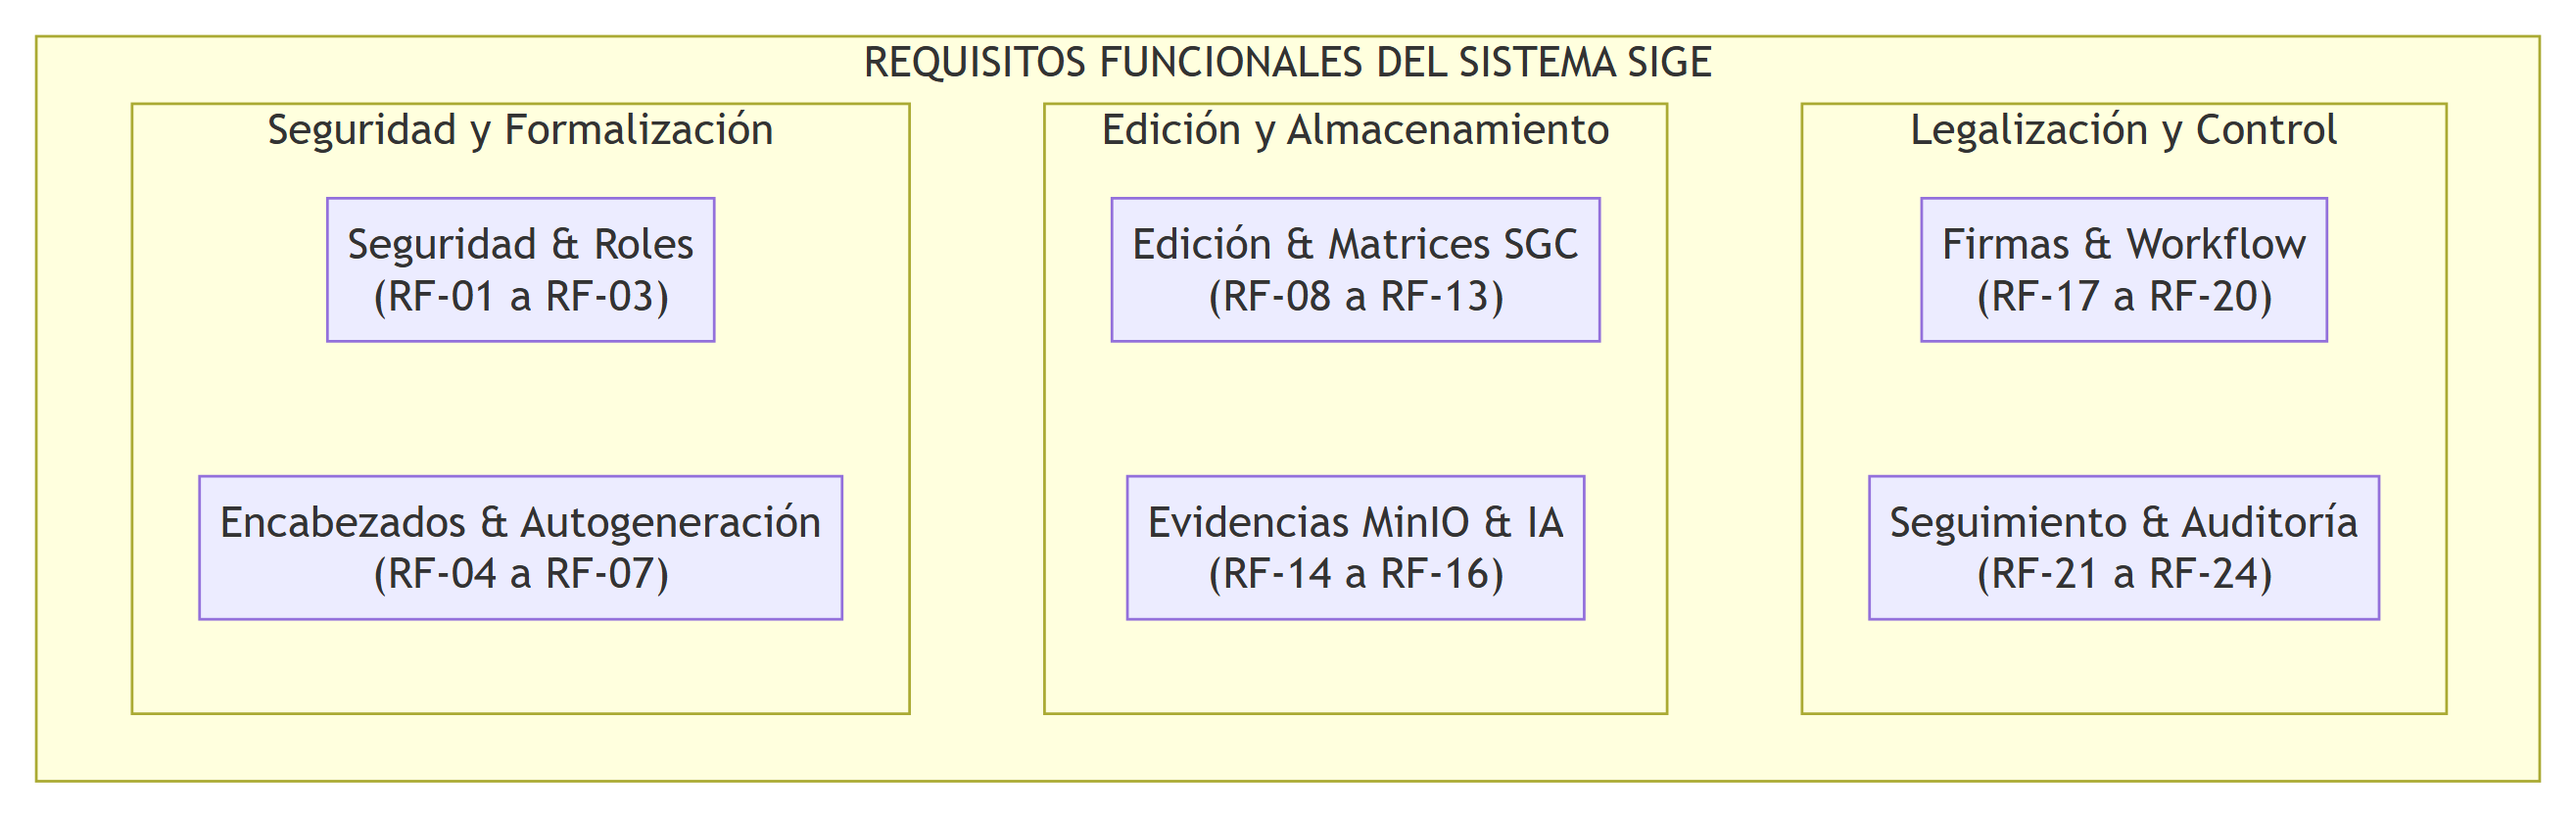
\includegraphics[width=0.88\textwidth,height=5.5cm,keepaspectratio]{images/s1_03_modulos_rf.png}
    \caption{Arquitectura Modular de Requerimientos Funcionales del Sistema SIGE.}
    \label{fig:s1_03_rf}
\end{figure}

\section{Descripción de actividades}
\subsection{Catálogo de Requerimientos Funcionales (RF-01 a RF-24)}

\begin{table}[htbp]
\centering
\footnotesize
\renewcommand{\arraystretch}{1.15}
\begin{tabularx}{\textwidth}{|c|>{\raggedright\arraybackslash\bfseries}m{2.6cm}|X|c|}
\hline
\rowcolor{tableheader}
\textbf{Código} & \textbf{Módulo} & \textbf{Descripción Funcional} & \textbf{Prioridad} \\
\hline
\textbf{RF-01} & Autenticación & Inicio de sesión seguro con credenciales institucionales y generación de JWT. & Alta \\
\hline
\textbf{RF-02} & Autenticación & Control de acceso basado en roles (Docente, Coordinador, Subdecano, Admin). & Alta \\
\hline
\textbf{RF-03} & Wizard Edición & Creación y gestión de borradores de Plan de Trabajo e Informe de Cumplimiento. & Alta \\
\hline
\textbf{RF-04} & Wizard Edición & Navegación modular por pestañas con validación previa de avance de paso. & Alta \\
\hline
\textbf{RF-05} & Editor TipTap & Edición de texto enriquecido para secciones descriptivas del formato SGC. & Alta \\
\hline
\textbf{RF-06} & Editor TipTap & Mecanismo de autoguardado asíncrono con debounce de 1500 ms y aviso visual. & Alta \\
\hline
\textbf{RF-07} & Matriz Dinámica & Registro dinámico de actividades académicas con horas y fechas de ejecución. & Alta \\
\hline
\textbf{RF-08} & Matriz Dinámica & Validación automática de suma de ponderaciones que obligue al 100\%. & Crítica \\
\hline
\textbf{RF-09} & Matriz Dinámica & Cálculo matemático ponderado en tiempo real del porcentaje de avance global. & Alta \\
\hline
\textbf{RF-10} & MinIO S3 & Carga en streaming de archivos PDF de evidencia hacia almacenamiento S3. & Alta \\
\hline
\textbf{RF-11} & MinIO S3 & Cálculo y persistencia del hash SHA-256 inmutable de cada archivo cargado. & Alta \\
\hline
\textbf{RF-12} & MinIO S3 & Generación de URLs prefirmadas de visualización segura con expiración de 60 min. & Media \\
\hline
\textbf{RF-13} & Validation Gates & Bloqueo preventivo de envío si el avance es mayor a 0\% y no hay evidencias. & Crítica \\
\hline
\textbf{RF-14} & Validation Gates & Validación de fechas de actividades contra el calendario académico oficial. & Alta \\
\hline
\textbf{RF-15} & Revisión Comité & Bandeja de revisión para Coordinadores de Área y Carrera con filtro por estado. & Alta \\
\hline
\textbf{RF-16} & Revisión Comité & Motor de observaciones granulares a nivel de sección o actividad específica. & Alta \\
\hline
\textbf{RF-17} & Cascada Firmas & Circuito de firmas de 3 niveles (Elaborador, Revisor, Aprobador) en serie. & Alta \\
\hline
\textbf{RF-18} & Cascada Firmas & Bloqueo de edición del documento una vez estampado el primer nivel de firma. & Crítica \\
\hline
\textbf{RF-19} & Corrección Texto & Integración con microservicio local LanguageTool para corrección ortográfica. & Media \\
\hline
\textbf{RF-20} & Asistencia Redacción & Asistencia de redacción académica formal mediante Google Gemini API. & Media \\
\hline
\textbf{RF-21} & Motor Exportación & Generación de archivos PDF oficiales idénticos a los formatos SGC P7-T1 y P7-T2. & Alta \\
\hline
\textbf{RF-22} & Motor Exportación & Generación de archivos DOCX editables con cabeceras y logos institucionales. & Media \\
\hline
\textbf{RF-23} & Auditoría & Registro inmutable de bitácora con estampas de tiempo, usuario y acción. & Alta \\
\hline
\textbf{RF-24} & Gestión Extemporánea & Solicitud y desbloqueo supervisado de edición fuera de plazo con justificación. & Media \\
\hline
\end{tabularx}
\caption{Catálogo de Requisitos Funcionales del Sistema SIGE.}
\label{tab:rf}
\end{table}

\subsection{Requisitos No Funcionales (RNF-01 a RNF-10)}
\begin{table}[htbp]
\centering
\small
\renewcommand{\arraystretch}{1.2}
\begin{tabularx}{\textwidth}{|c|>{\bfseries}m{2.8cm}|X|c|}
\hline
\rowcolor{tableheader}
\textbf{ID} & \textbf{Dimensión} & \textbf{Especificación Técnica} & \textbf{Métrica} \\
\hline
\textbf{RNF-01} & Rendimiento & Tiempo de respuesta de endpoints de persistencia y consultas. & $< 500$ ms \\
\hline
\textbf{RNF-02} & Rendimiento & Tiempo de generación y descarga de informes consolidados en PDF. & $< 3$ s \\
\hline
\textbf{RNF-03} & Seguridad & Cifrado de contraseñas con algoritmo bcrypt (factor de costo 10). & Inalterable \\
\hline
\textbf{RNF-04} & Seguridad & Tokens JWT firmados con HMAC-SHA256 y expiración máxima de 2 horas. & 120 min \\
\hline
\textbf{RNF-05} & Integridad & Hashes SHA-256 inmutables para toda evidencia almacenada en MinIO. & 256 bits \\
\hline
\textbf{RNF-06} & Disponibilidad & Disponibilidad de los servicios orquestados en contenedores Docker. & $99.5\%$ \\
\hline
\textbf{RNF-07} & Usabilidad & Diseño responsivo para pantallas móviles (375px) hasta escritorio (1920px). & CSS Fluido \\
\hline
\textbf{RNF-08} & Accesibilidad & Contraste cromático y navegación accesible según estándar WCAG 2.1. & Nivel AA \\
\hline
\textbf{RNF-09} & Mantenibilidad & Arquitectura modular desacoplada con separación estricta de capas. & Clean Arch \\
\hline
\textbf{RNF-10} & Portabilidad & Despliegue estandarizado de dependencias mediante Docker Compose. & Multiplataforma \\
\hline
\end{tabularx}
\caption{Especificación de Requisitos No Funcionales bajo ISO/IEC 25010.}
\label{tab:rnf}
\end{table}

\section{Firmas de Responsabilidad}

\noindent
\renewcommand{\arraystretch}{1.2}
\begin{tabularx}{\textwidth}{|>{\raggedright\arraybackslash}m{2.9cm}|>{\raggedright\arraybackslash}X|>{\centering\arraybackslash}m{4.6cm}|>{\centering\arraybackslash}m{2.3cm}|}
    \hline
    \rowcolor{tableheader}
    \textbf{ACCIÓN} & \textbf{NOMBRE Y CARGO} & \textbf{FIRMA} & \textbf{FECHA} \\
    \hline
    \textbf{Elaborado por:} & Heidi Villavicencio\newline Analista de Calidad / UI-UX & \parbox[c]{4.4cm}{\centering\vspace{4pt}
\includegraphics[height=1.5cm,width=4.0cm,keepaspectratio]{images/firma_heidi.png}\vspace{4pt}} & 21/08/2026 \\
    \hline
    \textbf{Revisado por:} & Steeven Toala\newline Líder de Proyecto / Arquitecto & \parbox[c]{4.4cm}{\centering\vspace{4pt}
\includegraphics[height=1.5cm,width=4.0cm,keepaspectratio]{images/firma_steveen.png}\vspace{4pt}} & 21/08/2026 \\
    \hline
    \textbf{Aprobado por:} & Ing. Paulo Torres, Mg.\newline Docente Evaluador -- Gestión Proyectos & \parbox[c]{4.4cm}{\centering\vspace{8pt}\textbf{\textcolor{gray!80}{\scriptsize [ PENDIENTE DE APROBACIÓN ]}}\vspace{8pt}} & \textbf{\textcolor{gray!90}{Pendiente}} \\
    \hline
\end{tabularx}

\vspace{0.4cm}

\section{Control de Cambios}

\noindent
\renewcommand{\arraystretch}{1.2}
\begin{tabularx}{\textwidth}{|>{\hsize=0.45\hsize\centering\arraybackslash}X|>{\hsize=1.55\hsize\raggedright\arraybackslash}X|>{\hsize=1.2\hsize\raggedright\arraybackslash}X|>{\hsize=0.8\hsize\centering\arraybackslash}X|}
    \hline
    \rowcolor{tableheader}
    \textbf{Versión} & \textbf{Descripción del cambio} & \textbf{Responsable del cambio} & \textbf{Fecha de aprobación} \\
    \hline
    1.0 & Emisión inicial del entregable según EDT del Tablero Trello & Equipo de Proyecto SIGE & 21/08/2026 \\
    \hline
\end{tabularx}

\vspace{0.4cm}

\section{Anexos}
\begin{itemize}[leftmargin=1.5em]
\item \textbf{Anexo 1:} Matriz de Trazabilidad Requisitos vs. Estándar SGC.
\end{itemize}

\end{document}
